\documentclass{beamer}

\usepackage{pgfplots}
\usepackage{pgfplotstable}
\usepackage{tikz}
\usepackage{xcolor}

\usepgfplotslibrary{fillbetween}
\usepgfplotslibrary{groupplots}

\usetikzlibrary{arrows}
\usetikzlibrary{arrows.meta}
\usetikzlibrary{calc}
\usetikzlibrary{positioning}

\usetheme{UiO}

\definecolor{ds002424}{HTML}{FF0028}
\definecolor{HBN}{HTML}{FF000E}
\definecolor{ABCD}{HTML}{FF0C00}
\definecolor{QTAB}{HTML}{FF2D00}
\definecolor{PING}{HTML}{FF4800}
\definecolor{ADHD200}{HTML}{FF6800}
\definecolor{PNC}{HTML}{FF8300}
\definecolor{ABIDE II}{HTML}{FFA400}
\definecolor{ds000119}{HTML}{FFBF00}\definecolor{ADHD}{HTML}{FF0028}
\definecolor{ANX}{HTML}{FF6E00}
\definecolor{ASD}{HTML}{F8FF00}
\definecolor{BIP}{HTML}{5BFF00}
\definecolor{DEM}{HTML}{00FF3B}
\definecolor{MCI}{HTML}{00FFD7}
\definecolor{MDD}{HTML}{008FFF}
\definecolor{MS}{HTML}{0E00FF}
\definecolor{PARK}{HTML}{A600FF}
\definecolor{SCZ}{HTML}{FF00BF}
\definecolor{HC}{HTML}{7F7F7F}
\definecolor{CoRR}{HTML}{15FF00}
\definecolor{HCP}{HTML}{00FF05}
\definecolor{FCON1000}{HTML}{00FF20}
\definecolor{ds000171}{HTML}{00FF40}
\definecolor{TOP}{HTML}{00FF5B}
\definecolor{SCZ-Z}{HTML}{00FF7B}
\definecolor{NIMH}{HTML}{00FF96}
\definecolor{NKI-RS}{HTML}{00FFB6}
\definecolor{MPI-LEMON}{HTML}{00FFD1}
\definecolor{ds003592}{HTML}{00FFF1}
\definecolor{ds004302}{HTML}{00F1FF}
\definecolor{ds000222}{HTML}{00D5FF}
\definecolor{SALD}{HTML}{00B5FF}
\definecolor{IXI}{HTML}{009AFF}
\definecolor{DLBS}{HTML}{0079FF}
\definecolor{Cam-CAN}{HTML}{005EFF}
\definecolor{StrokeMRI}{HTML}{003DFF}
\definecolor{PPMI}{HTML}{0022FF}
\definecolor{UKBB}{HTML}{0001FF}
\definecolor{Tao-Wu}{HTML}{1900FF}
\definecolor{ds000245}{HTML}{3400FF}
\definecolor{OASIS3}{HTML}{5500FF}
\definecolor{Demgen}{HTML}{7000FF}
\definecolor{NEUROCON}{HTML}{9000FF}
\definecolor{MIRIAD}{HTML}{AC00FF}
\definecolor{ds004392}{HTML}{CC00FF}
\definecolor{AIBL}{HTML}{E700FF}
\definecolor{ANM}{HTML}{FF00F5}
\definecolor{ADNI}{HTML}{FF00DA}

\definecolor{DEM}{HTML}{FF0028}
\definecolor{MS}{HTML}{FF6E00}
\definecolor{MCI}{HTML}{F8FF00}
\definecolor{SCZ}{HTML}{5BFF00}
\definecolor{ANX}{HTML}{00FF3B}
\definecolor{BIP}{HTML}{00FFD7}
\definecolor{ASD}{HTML}{008FFF}
\definecolor{MDD}{HTML}{0E00FF}
\definecolor{ADHD}{HTML}{A600FF}
\definecolor{HC}{HTML}{7F7F7F}

\title{Understanding the brain with explainable artificiall intelligence}
\subtitle{Detecting patterns of deviating brain aging in neuropsychiatric disorders}
\date{22.10.2024}
\author{Esten H. Leonardsen}


\begin{document}
    \begin{frame}
        \titlepage
    \end{frame}

    % \newcommand{\neuron}[2]{
    %     \node[
    %         circle,
    %         draw=black,
    %         fill=gray!50,
    %         minimum size=0.05cm,
    %         inner sep=0pt
    %     ] (#2) at ($ (side.north east) + (0.5, 0.5)  + #1 $){};
    % }

    % \newcommand{\stickman}[2]{
    %     \node[circle,fill,minimum size=2.5mm,#2] (head) at #1 {};
    %     \node[rounded corners=1pt,minimum height=0.65cm,minimum width=0.2cm,fill, below = 0.5pt of head,#2] (body) {};
    %     \draw[line width=0.5mm,round cap-round cap,#2] ([shift={(1pt,-0.5pt)}]body.north east) --++(-90:3mm);
    %     \draw[line width=0.5mm,round cap-round cap,#2] ([shift={(-1pt,-0.5pt)}]body.north west)--++(-90:3mm);
    %     \draw[thick,white,-round cap] (body.south) --++(90:2.75mm);
    % }

    % \newsavebox{\clinical}
    % \sbox{\clinical}{
    %     \begin{tikzpicture}
    %         \draw[dashed] (-1.6, 1.1) -- (0.8, -2.2);

    %         \stickman{(0, 0)}{red!80!blue}
    %         \stickman{(0.5, -0.5)}{red!95!blue}
    %         \stickman{(-0.4, 0.7)}{red!92!blue}
    %         \stickman{(1, 0.2)}{red}
    %         \stickman{(0.6, 0.9)}{red!75!blue}

    %         \stickman{(-0.5, -1)}{blue!80!red}
    %         \stickman{(-1.1, -0.8)}{blue!85!red}
    %         \stickman{(-1, 0.3)}{blue!75!red}
    %         \stickman{(0.1, -1.4)}{blue!95!red}
    %         \stickman{(-1.5, -0.1)}{blue}

    %         \node[font=\scriptsize\selectfont] at (-0.1, 1.3) {
    %             Patients
    %         };
    %         \node[font=\scriptsize\selectfont] at (-0.8, -2.1) {
    %             Controls
    %         };
    %     \end{tikzpicture}
    % }

    % \newsavebox{\population}
    % \sbox{\population}{
    %     \begin{tikzpicture}
    %         \stickman{(0, 0)}{blue}
    %         \stickman{(0.42, 0.4)}{blue!70!red}
    %         \stickman{(-0.42, 0.3)}{blue!95!red}
    %         \stickman{(-0.6, -0.8)}{blue!92!red}
    %         \stickman{(-0.15, -1.05)}{blue!65!red}
    %         \stickman{(0.4, -0.9)}{blue!91!red}
    %         \stickman{(0.87, -0.4)}{blue!98!red}
    %         \stickman{(-0.89, 0.4)}{blue!81!red}
    %         \stickman{(-1.35, -0.3)}{blue!87!red}
    %         \stickman{(-1, -1.2)}{blue!78!red}
    %         \stickman{(0.92, 0.7)}{blue!65!red}
    %         \stickman{(0.08, 1.1)}{blue!87!red}
    %         \stickman{(-0.35, 1.41)}{blue!80!red}
    %         \stickman{(-0.85, 1.54)}{blue!65!red}
    %         \stickman{(-1.31, 1.3)}{blue}
    %         \stickman{(0.5, 1.49)}{blue!99!red}
    %     \end{tikzpicture}
    % }

    % \newcommand{\brainageplot}[1]{
    %     \begin{tikzpicture}
    %         \begin{axis}[
    %             height=5cm,
    %             width=5cm,
    %             xlabel=\small{Chronological age},
    %             ylabel=\small{Apparent brain age},
    %             xmin=0,
    %             xmax=100,
    %             ymin=0,
    %             ymax=100,
    %             ticklabel style={font=\small},
    %             ylabel style={yshift=-0.2cm},
    %             xlabel style={yshift=0.05cm},
    %             ytick pos=left,
    %             xtick pos=bottom
    %         ]
    %             \addplot[dashed] coordinates {(0, 0) (100, 100)};

    %             \ifnum#1=0
    %                 \node[rotate=45, anchor=north, inner sep=1pt] at (axis cs: 68, 68) {
    %                     \tiny{Normative aging trajectory}
    %                 };
    %             \fi

    %             \ifnum#1=1
    %                 \draw[-stealth,densely dotted] (axis cs: 40, 40) -- (axis cs: 40, 58);
    %                 \draw[-stealth,densely dotted] (axis cs: 60, 60) -- (axis cs: 60, 42);
    %                 \addplot[
    %                     only marks,
    %                     mark=*,
    %                     draw=blue,
    %                     fill=blue!50
    %                 ] coordinates {
    %                     (40, 60)
    %                     (60, 40)
    %                 };
    %                 \node[
    %                     font=\scriptsize\linespread{0.8}\selectfont,
    %                     anchor=south,
    %                     align=center
    %                 ] at (axis cs: 40, 60) {
    %                     Older\\appearing\\brain
    %                 };
    %                 \node[
    %                     font=\scriptsize\linespread{0.8}\selectfont,
    %                     anchor=north,
    %                     align=center
    %                 ] at (axis cs: 60, 40) {
    %                     Younger\\appearing\\brain
    %                 };

    %             \fi
    %         \end{axis}
    %     \end{tikzpicture}
    % }

    % \newsavebox{\brainage}
    % \sbox{\brainage}{
    %     \brainageplot{0}
    % }

    % \newsavebox{\brainagepredictions}
    % \sbox{\brainagepredictions}{
    %     \brainageplot{1}
    % }

    % \begin{frame}{Motivation}
    %     \begin{tikzpicture}
    %         \node[draw=black] at (-5.25, -3.5) {};
    %         \node[draw=black] at (5.25, 3.5) {};

    %         \visible<1>{
    %             \node[] at (0, 0) {
    %                 Cognitive neuroscience
    %             };
    %         }
    %         \visible<2>{
    %             \node[] at (0, 0) {
    %                 Brain complexity
    %             };
    %         }
    %         \visible<3-7>{
    %             \node[anchor=east] (threed) at (4.5, 2) {
    %                 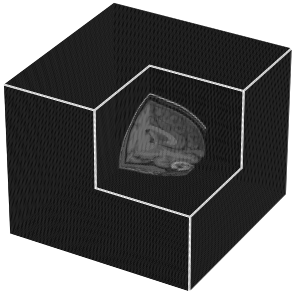
\includegraphics[height=3cm]{data/3d_bert.png}
    %             };
    %         }
    %         \visible<3-6>{
    %             \node[
    %                 font=\fontsize{10}{10}\selectfont\bfseries,
    %                 align=center,
    %                 anchor=west
    %             ] at (-4.5, 2) {
    %                 Structural Magnetic\\
    %                 Resonance Imaging (MRI) scans
    %             };

    %             \node[label=below:\small{Side}] (side) at (-3.25, -1.65) {
    %                 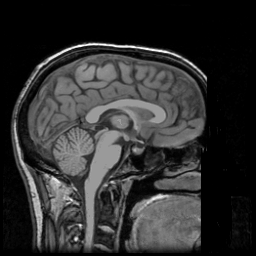
\includegraphics[height=2.5cm]{data/bert_x_enhanced.png}
    %             };

    %             \node[label=below:\small{Above}] at (0, -1.65) {
    %                 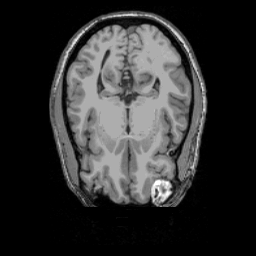
\includegraphics[height=2.5cm]{data/bert_y_enhanced.png}
    %             };

    %             \node[label=below:\small{Front}] at (3.25, -1.65) {
    %                 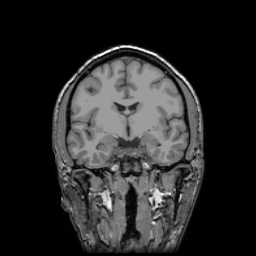
\includegraphics[height=2.5cm]{data/bert_z_enhanced.png}
    %             };
    %         }
    %         \visible<4-5>{
    %             \node[] at ($ (side.north east) + (0.5, 0.5) $) {
    %                 
\includegraphics[width=3cm]{data/region.png}
    %             };
    %             \node[
    %                 draw=red,
    %                 circle,
    %                 minimum size=3cm,
    %                 thick
    %             ] at ($ (side.north east) + (0.495, 0.495) $) {};
    %             \node[
    %                 draw=red,
    %                 circle,
    %                 minimum size=0.05cm,
    %                 inner sep=0pt,
    %             ] at ($ (side.north east) - (1.2, 1.12) $) {};
    %             \draw[red] ($ (side.north east) - (1.225, 1.12) $) --
    %                        ($ (side.north east) - (0.99, -0.75) $);
    %             \draw[red] ($ (side.north east) - (1.2, 1.145) $) --
    %                        ($ (side.north east) - (-0.75, 0.99) $);
    %         }
    %         \visible<5>{
    %             \node[
    %                 draw=red,
    %                 minimum height=0.6cm,
    %                 minimum width=0.6cm
    %             ] at ($ (side.north east) + (0.5, 0.5) $) {};

    %             \neuron{(0.1, 0.1)}{n0}
    %             \neuron{(0.05, 0.15)}{n1}
    %             \neuron{(-0.2, -0.1)}{n2}
    %             \neuron{(-0.15, 0.1)}{n3}
    %             \neuron{(0, -0.05)}{n4}
    %             \neuron{(0.13, -0.21)}{n5}
    %             \neuron{(0.15, -0.02)}{n6}
    %             \neuron{(-0.08, -0.13)}{n7}
    %             \neuron{(-0.05, 0.22)}{n8}

    %             \pgfplotsforeachungrouped  \i in {0,...,8} {
    %                 \pgfplotsforeachungrouped  \j in {0,...,8} {
    %                     \ifdim\i pt<\j pt
    %                         \draw[line width=0.25pt] (n\i) -- (n\j);
    %                     \fi
    %                 }
    %             }

    %             \neuron{(0.1, 0.1)}{n0}
    %             \neuron{(0.05, 0.15)}{n1}
    %             \neuron{(-0.2, -0.1)}{n2}
    %             \neuron{(-0.15, 0.1)}{n3}
    %             \neuron{(0, -0.05)}{n4}
    %             \neuron{(0.13, -0.21)}{n5}
    %             \neuron{(0.15, -0.02)}{n6}
    %             \neuron{(-0.08, -0.13)}{n7}
    %             \neuron{(-0.05, 0.22)}{n8}

    %         }
    %         \visible<6-7>{
    %             \node[rotate=-14, font=\small\selectfont] (label1) at ($ (threed) + (0.545, 1.46) $) {256};
    %             \node[rotate=37, font=\small\selectfont] (label2) at ($ (threed) + (-0.915, 1.3) $) {256};
    %             \node[rotate=93, font=\small\selectfont] (label3) at ($ (threed) - (1.67, 0.115) $) {256};
    %             \node[font=\boldmath] at ($ (threed.south) + (0, -0.2) $) {
    %                 $p \approx 10\,000\,000$
    %             };
    %         }
    %         \visible<7-8>{
    %             \node[] (clinical) at (-3, 0) {
    %                 \usebox{\clinical}
    %             };
    %             \node[anchor=north, align=center, font=\small\selectfont\bfseries\boldmath] at (clinical.south) {
    %                 Clinical datasets\\
    %                 ($n \approx 100$)
    %             };
    %         }
    %         \visible<8>{
    %             \node[] (population) at (3, 0) {
    %                 \usebox{\population}
    %             };
    %             \node[anchor=north, align=center, font=\small\selectfont\bfseries\boldmath] at (population.south) {
    %                 Population datasets\\
    %                 ($n \approx 10\,000$)
    %             };
    %         }
    %         \visible<9-11>{
    %             \node[anchor=west, label={[label distance=-0.15cm, anchor=north]below:\scriptsize{Generated by Dall-E 3}}] at (-5.1, 0) {
    %                 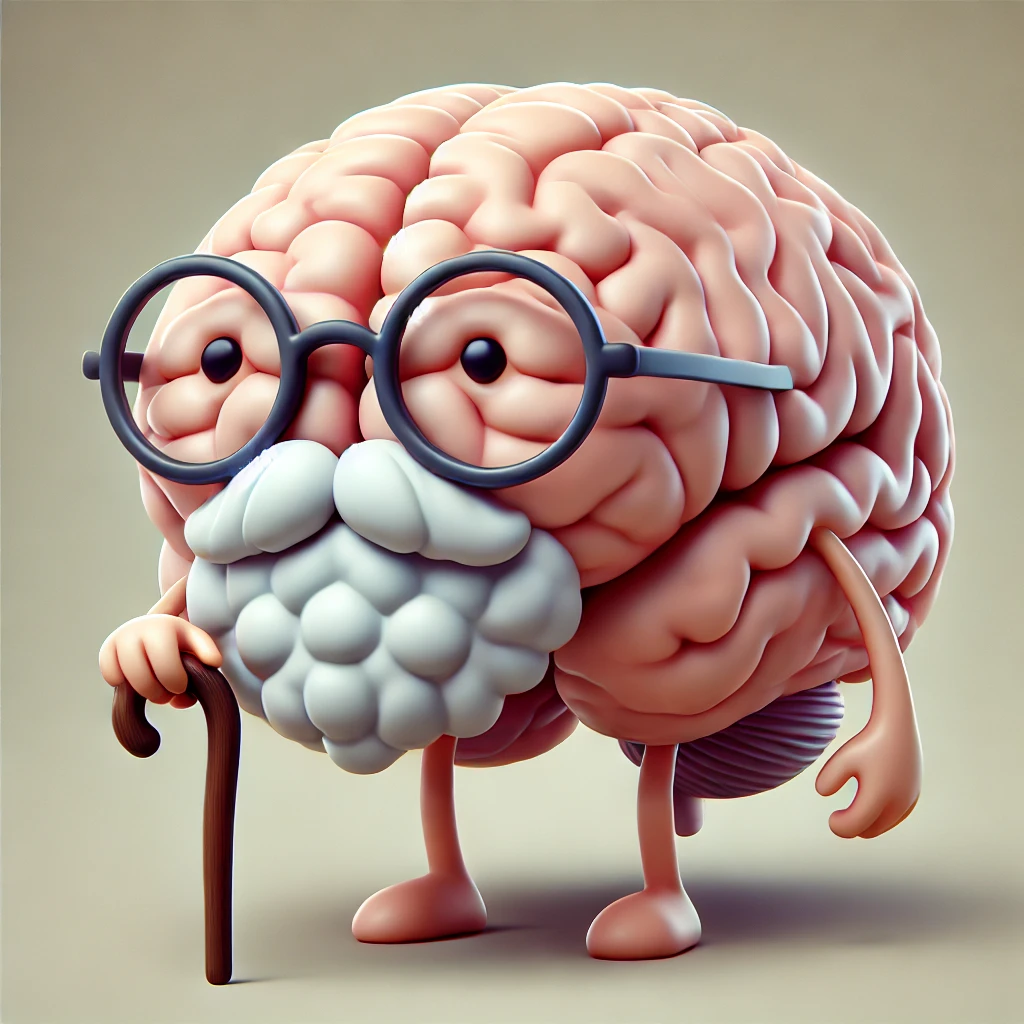
\includegraphics[width=4cm]{data/brainage.png}
    %             };
    %         }
    %         \visible<10>{
    %             \node[anchor=east] at (5.1, -0.43) {
    %                 \usebox{\brainage}
    %             };
    %         }
    %         \visible<11>{
    %             \node[anchor=east] at (5.1, -0.43) {
    %                 \usebox{\brainagepredictions}
    %             };
    %         }
    %     \end{tikzpicture}
    % \end{frame}

    % \newsavebox{\datasetbox}
    % \sbox{\datasetbox}{
    %     \begin{tikzpicture}
    %         \pgfplotstableread[col sep=comma]{data/full_data_distributions.csv}\data

    %         \begin{axis}[
    %             width=0.8\textwidth,
    %             height=0.85\textwidth,
    %             xmin=0,
    %             xmax=100,
    %             ytick=\empty,
    %             axis x line=middle,
    %             axis y line=none,
    %             xtick={10,20,30,40,50,60,70,80},
    %             x axis line style={|-stealth},
    %             clip=false
    %         ]
    %             \addplot[
    %                 name path global=zero,
    %             ] coordinates {(0,0) (100,0)};

    %             \def\previouspath{zero}

    %             \pgfplotsforeachungrouped \sex/\sign in {female/1, male/-1} {
    %                 \xdef\previouspath{zero}
    %                 % \pgfplotsforeachungrouped \dataset in {ds002424, HBN, ABCD, QTAB, PING, ADHD200, PNC, {ABIDE II}, ds000119,{ABIDE I}, BRAINMINT, SLIM, QTIM, Beijing, AOMIC-PIOP2, ds000202, AOMIC-PIOP1, CoRR, HCP, FCON1000, ds000171, TOP, SCZ-Z, NIMH, NKI-RS, MPI-LEMON, ds003592, ds004302, ds000222, SALD, IXI, DLBS, Cam-CAN, StrokeMRI, PPMI, UKBB, Tao-Wu, ds000245, OASIS3, Demgen, NEUROCON, MIRIAD, ds004392, AIBL, ANM, ADNI} {
    %                 \pgfplotsforeachungrouped \dataset in {ds002424, HBN, ABCD} {
    %                     \edef\currentpath{\sex\dataset}
    %                     \edef\currentfill{\dataset!50}
    %                     \edef\region{\previouspath\space and\space\currentpath}

    %                     \addplot [
    %                         draw=none,
    %                         line width=0pt,
    %                         name path global={\currentpath},
    %                     ] table [
    %                         x=age,
    %                         y expr=\sign * \thisrow{\sex_\dataset}
    %                     ]{\data};

    %                     \addplot[
    %                         fill=\currentfill
    %                     ] fill between [
    %                         of/.expanded={\region}
    %                     ];

    %                     \typeout{\region}
    %                 }
    %             }

    %             \node[
    %                 circle,
    %                 anchor=west,
    %                 draw=ds002424,
    %                 fill=ds002424!50,
    %                 label={[text depth=0]right:\footnotesize{ds002424}},
    %                 inner sep=2pt
    %             ] (legend1) at (axis cs: 102, 1){};
    %         \end{axis}
    %     \end{tikzpicture}
    % }

    \newcommand{\inputfront}[2]{
        \def\mridepth{0.6}
        \node[yslant=1, inner sep=0pt] (input) at (#1, #2) {
            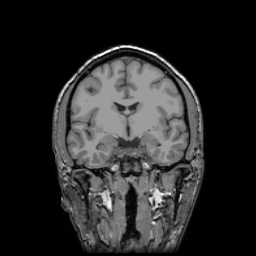
\includegraphics[height=1.7cm, width=1cm]{data/bert_z_enhanced.png}
        };
        \draw[fill=black] (input.north east) --
            ($ (input.north east) - (\mridepth, 0) $) --
            ($ (input.north west) - (\mridepth, 0) $) --
            (input.north west) -- cycle;
        \draw[fill=black] (input.north west) --
            ($ (input.north west) - (\mridepth, 0) $) --
            ($ (input.south west) - (\mridepth, 0) $) --
            (input.south west) -- cycle;
        \draw[] (input.north east) --
            ($ (input.north east) + (\mridepth, 0) $) --
            ($ (input.north west) + (\mridepth, 0) $) --
            (input.north west) -- cycle;
        \draw[]  ($ (input.north west) + (\mridepth, 0) $) --
            ($ (input.south west) + (\mridepth, 0) $) --
            (input.south west);
        \draw[] ($ (input.north east) + (\mridepth, 0) $) --
            ($ (input.south east) + (\mridepth, 0) $) --
            ($ (input.south west) + (\mridepth, 0) $);
    }

    \newcommand{\mritop}[3]{
        \def\mridepth{0.75}

        \node[inner sep=0pt, xslant=1] (input) at (#1, #2) {
            \includegraphics[height=1.5cm, width=0.75cm, rotate=90]{#3}
        };
        \draw[fill=black] (input.north east) --
            ($ (input.north east) - (0, \mridepth) $) --
            ($ (input.south east) - (0, \mridepth) $) --
            (input.south east) -- cycle;
        \draw[fill=black] (input.south west) --
            ($ (input.south west) - (0, \mridepth) $) --
            ($ (input.south east) - (0, \mridepth) $) --
            (input.south east) -- cycle;
        \draw[] (input.south west) --
            ($ (input.south west) + (0, \mridepth) $) --
            ($ (input.north west) + (0, \mridepth) $) --
            (input.north west) -- cycle;
        \draw[] (input.south east) --
            ($ (input.south east) + (0, \mridepth) $) --
            ($ (input.north east) + (0, \mridepth) $) --
            (input.north east) -- cycle;
        \draw[] ($ (input.south east) + (0, \mridepth) $) --
            ($ (input.south west) + (0, \mridepth) $);
        \draw[] ($ (input.north east) + (0, \mridepth) $) --
            ($ (input.north west) + (0, \mridepth) $);
    }

    \newcommand{\inputtop}[2]{
        \mritop{#1}{#2}{data/bert_y_enhanced.png}
    }

    \newcommand{\segmentationtop}[2]{
        \mritop{#1}{#2}{data/segmentation.png}
    }

    \newcommand{\mriside}[3]{
        \def\mridepth{0.75}

        \node[inner sep=0pt] (input) at (#1, #2) {
            \includegraphics[height=1.5cm, width=1.5cm]{#3}
        };

        \draw[fill=black] (input.north west) --
            ($ (input.north west) + (0.5 * \mridepth, 0.5 * \mridepth) $) --
            ($ (input.north east) + (0.5 * \mridepth, 0.5 * \mridepth) $) --
            (input.north east) -- cycle;
        \draw[fill=black] (input.north east) --
            ($ (input.north east) + (0.5 * \mridepth, 0.5 * \mridepth) $) --
            ($ (input.south east) + (0.5 * \mridepth, 0.5 * \mridepth) $) --
            (input.south east) -- cycle;
        \draw[] (input.north west) --
            ($ (input.north west) - (0.5 * \mridepth, 0.5 * \mridepth) $) --
            ($ (input.south west) - (0.5 * \mridepth, 0.5 * \mridepth) $) --
            (input.south west) -- cycle;
        \draw[] (input.north east) --
            ($ (input.north east) - (0.5 * \mridepth, 0.5 * \mridepth) $) --
            ($ (input.south east) - (0.5 * \mridepth, 0.5 * \mridepth) $) --
            (input.south east) -- cycle;
        \draw[] ($ (input.north west) - (0.5 * \mridepth, 0.5 * \mridepth) $) --
            ($ (input.north east) - (0.5 * \mridepth, 0.5 * \mridepth) $);
        \draw[] ($ (input.south west) - (0.5 * \mridepth, 0.5 * \mridepth) $) --
            ($ (input.south east) - (0.5 * \mridepth, 0.5 * \mridepth) $);
    }

    \newcommand{\inputside}[2]{
        \mriside{#1}{#2}{data/bert_x_enhanced.png}
    }

    \newcommand{\segmentationside}[2]{
        \mriside{#1}{#2}{data/segmentation.png}
    }

    \newcommand{\heatmapside}[2]{
        \segmentationside{#1}{#2}
    }

    \newcommand{\convside}[6]{
        \def\sidex{#1}
        \def\sidey{#2}
        \def\sidewidth{#3}
        \def\sideheight{#4}
        \def\sidefillcolour{#5}
        \def\sidename{#6}

        \node[
            fill=\sidefillcolour,
            inner sep=0pt,
            outer sep=0pt,
            minimum width=\sidewidth,
            minimum height=\sideheight,
            draw=black
        ] (\sidename) at (\sidex, \sidey) {};
    }

    \newcommand{\convtop}[4]{
        \def\topbase{#1}
        \def\topwidth{#2}
        \def\topheight{#3}
        \def\topfillcolour{#4}

        \draw[fill=\topfillcolour,draw=black] #1 --
            ($ #1 + (#3, #3) $) --
            ($ #1 + (#3+#2, #3) $) --
            ($ #1 + (#2, 0) $);
    }

    \newcommand{\convfront}[3]{
        \def\frontbase{#1}
        \def\frontsize{#2}
        \def\frontfillcolour{#3}

        \draw[black, fill=\frontfillcolour] #1 --
            ($ #1 + (1*#2, 1*#2) $) --
            ($ #1 + (1*#2, 1*#2 - 2*#2) $) --
            ($ #1 + (0, -2*#2) $);
    }


    \newcommand{\convchannel}[7]{
        \def\channelx{#1}
        \def\channely{#2}
        \def\channelnodedepth{#3}
        \def\channelnodesize{#4}
        \def\channelnodecount{#5}
        \def\channelcolour{#6}
        \def\includefront{#7}

        \def\huemin{20}
        \def\huemax{80}

        \pgfmathsetmacro{\iterations}{#5-1}
        \foreach \i in {0,...,\iterations} {
            \pgfmathsetmacro{\hue}{int(random(\huemin, \huemax))}
            \convside{#1}{#2+\i*-#4}{#3 cm}{#4 cm}{#6!\hue}{n\i0}

            \foreach \j in {0,...,\iterations} {
                \pgfmathsetmacro{\innerhue}{int(random(\huemin, \huemax))}
                \ifnum\j=0
                    \pgfmathsetmacro{\innerhue}{\hue}
                \fi

                \ifnum\includefront=1
                    \convfront{($ (n00.north east) + (0.5*\j*#4, 0.5*\j*#4 - \i*#4) $)}{0.5*#4}{#6!\innerhue}
                \fi

                \ifnum\i=0
                    \convtop{($ (n\i0.north west) + (0.5*\j*#4, 0.5*\j*#4) $)}{#3}{0.5*#4}{#6!\innerhue}
                \fi
            }
        }
    }

    \newcommand{\lrpchannel}[6]{
        \def\channelx{#1}
        \def\channely{#2}
        \def\channelnodedepth{#3}
        \def\channelnodesize{#4}
        \def\channelnodecount{#5}
        \def\includefront{#6}

        \colorlet{bgcolour}{black!85}

        \pgfmathsetmacro{\iterations}{#5-1}
        \foreach \i in {0,...,\iterations} {
            \pgfmathsetmacro{\hue}{int(random(-150, 100))}
            \colorlet{fillcolour}{bgcolour}

            \colorlet{lrpcolour}{red}
            \pgfmathsetmacro{\coinflip}{int(random(0, 1))}

            \ifnum\coinflip=1
                \colorlet{lrpcolour}{blue}
            \fi

            \ifnum\hue>0
                \colorlet{fillcolour}{lrpcolour!\hue!bgcolour}
            \fi

            \convside{#1}{#2+\i*-#4}{#3 cm}{#4 cm}{fillcolour}{n\i0}

            \foreach \j in {0,...,\iterations} {
                \pgfmathsetmacro{\innerhue}{int(random(-150, 100))}
                \colorlet{innerfillcolour}{bgcolour}

                \ifnum\innerhue>0
                    \colorlet{innerfillcolour}{lrpcolour!\innerhue!bgcolour}
                \fi

                \ifnum\j=0
                    \colorlet{innerfillcolour}{fillcolour}
                \fi

                \ifnum\includefront=1
                    \convfront{($ (n00.north east) + (0.5*\j*#4, 0.5*\j*#4 - \i*#4) $)}{0.5*#4}{innerfillcolour}
                \fi

                \ifnum\i=0
                    \convtop{($ (n\i0.north west) + (0.5*\j*#4, 0.5*\j*#4) $)}{#3}{0.5*#4}{innerfillcolour}
                \fi
            }
        }
    }

    \newcommand{\convlayer}[7]{
        \def\layerx{#1}
        \def\layery{#2}
        \def\layernodedepth{#3}
        \def\layernodesize{#4}
        \def\layernodecount{#5}
        \def\layerdepth{#6}
        \def\layercolour{#7}

        \pgfmathsetmacro{\layeriterations}{\layerdepth-1}
        \foreach \i in {0,...,\layeriterations}{
            \pgfmathsetmacro{\x}{\layerx + \i * \layernodedepth}
            \pgfmathsetmacro{\islast}{\i == \layeriterations ? 1 : 0}
            \convchannel{\x}{\layery}{\layernodedepth}{\layernodesize}{\layernodecount}{\layercolour}{\islast}
        }
    }

    \newcommand{\lrplayer}[6]{
        \def\layerx{#1}
        \def\layery{#2}
        \def\layernodedepth{#3}
        \def\layernodesize{#4}
        \def\layernodecount{#5}
        \def\layerdepth{#6}

        \pgfmathsetmacro{\layeriterations}{\layerdepth-1}
        \foreach \i in {0,...,\layeriterations}{
            \pgfmathsetmacro{\x}{\layerx + \i * \layernodedepth}
            \pgfmathsetmacro{\islast}{\i == \layeriterations ? 1 : 0}
            \lrpchannel{\x}{\layery}{\layernodedepth}{\layernodesize}{\layernodecount}{\islast}
        }
    }

    \newcommand{\modelarrow}[5]{
        \begin{scope}[transparency group, opacity=0.5]
            \draw[-stealth, line width=2pt, #3] #1 to [in=#4, out=#5] #2;
        \end{scope}
    }

    \newcommand{\cnnarrow}[3]{
        \modelarrow{#1}{#2}{#3}{180}{0}
    }

    \newcommand{\lrparrow}[3]{
        \modelarrow{#1}{#2}{#3}{0}{180}
    }

    \newcommand{\cnn}[6]{
        \def\xmin{#1}
        \def\ymin{#2}
        \def\nodedepth{#3}
        \def\nodesize{#4}
        \def\modelcolour{#5}
        \def\annotate{#6}

        \convlayer{#1 - 0.06 + 0.4}{#2 + 2.5 * #4}{#3}{#4}{12}{3}{\modelcolour}
        \cnnarrow{(#1 + 0.95, #2)}{(#1+2.2, #2)}{#5}

        \convlayer{#1 + 1.44 + 0.4}{#2 + 1.5 * #4}{#3}{#4}{8}{5}{\modelcolour}
        \cnnarrow{(#1 + 2.43, #2)}{(#1+3.5, #2)}{#5}

        \convlayer{#1 + 2.77 + 0.4}{#2 + 0.5 * #4}{#3}{#4}{4}{7}{\modelcolour}
        \cnnarrow{(#1 + 3.75, #2)}{(#1+5, #2)}{#5}

        \convlayer{#1 + 3.93 + 0.4}{#2 + 0}{#3}{#4}{2}{9}{\modelcolour}

        \ifdim #6 pt = 1 pt
            \draw[thick, dashed] (#1 + 0.22, #2 + 1.43) --
                                (#1 + 5.13, #2 + 1.43) --
                                (#1 + 5.13, #2 - 1.42) --
                                (#1 + 0.22, #2 - 1.42) -- cycle;
            \node[anchor=south, text depth=0, font=\small\selectfont] at (#1 + 2.675, #2 + 1.43) {
                \textbf{3D Convolutional Neural Network}
            };
        \fi
    }

    \newcommand{\lrp}[4]{
        \def\xmin{#1}
        \def\ymin{#2}
        \def\nodedepth{#3}
        \def\nodesize{#4}

        \lrplayer{#1 - 0.06 + 0.4}{#2 + 2.5 * #4}{#3}{#4}{12}{3}{black}
        \lrparrow{(#1+2.2, #2)}{(#1 + 0.95, #2)}{black}

        \lrplayer{#1 + 1.44 + 0.4}{#2 + 1.5 * #4}{#3}{#4}{8}{5}{black}
        \lrparrow{(#1+3.5, #2)}{(#1 + 2.43, #2)}{black}

        \lrplayer{#1 + 2.77 + 0.4}{#2 + 0.5 * #4}{#3}{#4}{4}{7}{black}
        \lrparrow{(#1+5, #2)}{(#1 + 3.75, #2)}{black}

        \lrplayer{#1 + 3.93 + 0.4}{#2 + 0}{#3}{#4}{2}{9}{black}
    }

    \newcommand{\cnnbox}[1]{
        \definecolor{hippocampus}{HTML}{74c476}
        \definecolor{thalamus}{HTML}{e6550d}
        \definecolor{cortex}{HTML}{7eaaf1}

        \begin{tikzpicture}
            \node[draw=black] at (-2.5, 0) {};
            \node[draw=black] at (7.6, 0) {};


            \ifnum#1=0
                \node[
                    font=\small\linespread{0.9}\selectfont,
                    align=center,
                    anchor=west
                ] (output) at (5.35, 0) {
                    Chronological\\age
                };
            \fi
            \ifnum#1=1
                \node[
                    font=\small\linespread{0.9}\selectfont,
                    align=center,
                    anchor=west
                ] (output) at (5.35, 0) {
                    Apparent\\brain age
                };
            \fi
            \ifnum#1=3
                \node[
                    font=\small\linespread{0.9}\selectfont,
                    align=center,
                    anchor=west
                ] (output) at (5.35, 0) {
                    Apparent\\brain age
                };
            \fi

            \ifnum#1<2
                \inputside{-1.4}{0}
                \cnnarrow{(input.east)}{($ (input.center) + (2, 0) $)}{black}
            \fi
            \ifnum#1=0
                \cnn{0}{0}{0.066}{0.15}{black}{1}
            \fi
            \ifnum#1=1
                \cnn{0}{0}{0.066}{0.15}{black}{0}
            \fi
            \ifnum#1<2
                \cnnarrow{($ (output.west) - (0.39, 0) $)}{($ (output.west) + (0.1, 0) $)}{black}
            \fi

            \ifnum#1=2
                \segmentationside{-1.4}{0}

                \cnnarrow{(input.east)}{($ (input.center) + (2, 2) $)}{cortex}
                \cnnarrow{(input.east)}{($ (input.center) + (2, 0) $)}{hippocampus}
                \cnnarrow{(input.east)}{($ (input.center) + (2, -2) $)}{thalamus}

                \cnn{0}{2}{0.066}{0.1}{cortex}{0}
                \cnn{0}{0}{0.066}{0.1}{hippocampus}{0}
                \cnn{0}{-2}{0.066}{0.1}{thalamus}{0}

                \node[
                    font=\footnotesize\linespread{0.9}\selectfont,
                    align=center,
                    anchor=west
                ] (output0) at (5.35, 2) {
                    Apparent\\cortical age
                };
                \node[
                    font=\footnotesize\linespread{0.9}\selectfont,
                    align=center,
                    anchor=west
                ] (output1) at (5.35, 0) {
                    Apparent\\hippocampal\\age
                };
                \node[
                    font=\footnotesize\linespread{0.9}\selectfont,
                    align=center,
                    anchor=west
                ] (output2) at (5.35, -2) {
                    Apparent\\thalamic age
                };

                \cnnarrow{($ (output0.west) - (0.39, 0) $)}{($ (output0.west) + (0.1, 0) $)}{cortex}
                \cnnarrow{($ (output1.west) - (0.39, 0) $)}{($ (output1.west) + (0.1, 0) $)}{hippocampus}
                \cnnarrow{($ (output2.west) - (0.39, 0) $)}{($ (output2.west) + (0.1, 0) $)}{thalamus}
            \fi

            \ifnum#1=3
                \heatmapside{-1.4}{0}

                \lrp{0}{0}{0.066}{0.15}

                \lrparrow{($ (input.center) + (2, 0) $)}{(input.east)}{black}
                \lrparrow{($ (output.west) + (0.1, 0) $)}{($ (output.west) - (0.39, 0) $)}{black}
            \fi
        \end{tikzpicture}
    }

    \newsavebox{\cnntraining}
    \sbox{\cnntraining}{
        \cnnbox{0}
    }

    \newsavebox{\cnnforward}
    \sbox{\cnnforward}{
        \cnnbox{1}
    }

    \newsavebox{\cnnregions}
    \sbox{\cnnregions}{
        \cnnbox{2}
    }

    \newsavebox{\cnnlrp}
    \sbox{\cnnlrp}{
        \cnnbox{3}
    }

    % \newsavebox{\results}
    % \sbox{\results}{
    %     \begin{tikzpicture}
	% 		\begin{axis}[
	% 			xmin=0,
	% 			xmax=100,
	% 			ymin=0,
	% 			ymax=100,
	% 			xtick pos=bottom,
	% 			ytick pos=left,
	% 			xlabel={Chronological age},
	% 			ylabel={Predicted brain age},
    %             height=7cm,
    %             width=7cm
	% 		]
	% 			\addplot [red] coordinates {(0,0) (100,100)};
	% 			\addplot [
	% 				only marks,
	% 				mark size=2pt,
	% 				color=blue,
	% 				opacity=0.2
	% 			] table [
	% 				x=yhat,
	% 				y=y,
	% 				col sep=comma
	% 			] {data/predictions.csv};
	% 			\addplot [red] coordinates {(0,0) (100,100)};
	% 			\node [anchor=south east,inner sep=0pt,outer sep=0pt] (outofsample) at (rel axis cs:0.92,0.08) {\textcolor{red}{MAE=4.73}};
	% 		\end{axis}
	% 	\end{tikzpicture}
    % }

    \newcommand{\disorderplot}[3]{
        \nextgroupplot[
            xticklabels={#2},
            xlabel={#3}
        ]
            \addplot [
                draw=none,
                line width=0pt,
                name path=zero,
            ] coordinates {(0,0) (15,0)};

            \addplot [
                draw=none,
                line width=0pt,
                name path=#1-HC,
            ] table [
                col sep=comma,
                x=x,
                y=#1-HC
            ] {data/disorders.csv};

            \addplot[
                HC,
                opacity=0.75,
            ] fill between [
                of=zero and #1-HC
            ];

            \addplot [
                draw=none,
                line width=0pt,
                name path=#1,
            ] table [
                col sep=comma,
                x=x,
                y=#1
            ] {data/disorders.csv};

            \addplot[
                #1,
                opacity=0.75,
            ] fill between [
                of=zero and #1
            ];
    }

    \newsavebox{\patients}
    \sbox{\patients}{
        \newcommand{\legendnode}[4]{
            \node[align=left, font=\tiny\selectfont, anchor=west] at #1 {
                \textbf{#2}\\
                $\Delta$=#3 (p=$#4$)
            };
        }
        \begin{tikzpicture}
            \begin{groupplot}[
                group style={
                    group size=1 by 9,
                    vertical sep=0.05cm,
                    group name=group
                },
                height=2.23cm,
                width=10cm,
                xmin=-15,
                xmax=15,
                ymax=1,
                ymin=0,
                ytick=\empty,
                axis x line=bottom,
                xtick={-10,0,10},
                xticklabels=\empty,
                axis y line=none,
                x axis line style={stealth-stealth},
                clip=false,
                xticklabel style={font=\footnotesize},
                xlabel style={font=\footnotesize, yshift=0.15cm},
            ]
                \disorderplot{DEM}{\empty}{}
                \disorderplot{MS}{\empty}{}
                \disorderplot{MCI}{\empty}{}
                \disorderplot{SCZ}{\empty}{}
                \disorderplot{ANX}{\empty}{}
                \disorderplot{BIP}{\empty}{}
                \disorderplot{ASD}{\empty}{}
                \disorderplot{MDD}{\empty}{}
                \disorderplot{ADHD}{{-10,0,10}}{Brain age delta}

            \end{groupplot}
            \legendnode{($ (group c1r1.west) + (0, 0) $)}{Dementia}{5.10}{2.53\times10^{-48}}
            \legendnode{($ (group c1r2.west) + (0, 0) $)}{Multiple sclerosis}{3.82}{1.35\times10^{-9}}
            \legendnode{($ (group c1r3.west) + (0, 0) $)}{Mild cognitive impairment}{1.75}{7.64\times10^{-8}}
            \legendnode{($ (group c1r4.west) + (0, 0) $)}{Schizophrenia}{1.26}{4.34\times10^{-4}}
            \legendnode{($ (group c1r5.west) + (0, 0) $)}{Anxiety disorder}{1.00}{0.17}
            \legendnode{($ (group c1r6.west) + (0, 0) $)}{Bipolar disorder}{0.86}{0.04}
            \legendnode{($ (group c1r7.west) + (0, 0) $)}{Autism spectrum disorder}{0.38}{0.20}
            \legendnode{($ (group c1r8.west) + (0, 0) $)}{Major depressive disorder}{0.08}{0.93}
            \legendnode{($ (group c1r9.west) + (0, 0) $)}{Attention deficit/hyperactivity disorder}{-0.07}{0.81}
        \end{tikzpicture}
    }

    \newcommand{\dementiaplot}[1]{
        \begin{tikzpicture}
            \begin{axis}[
                height=5cm,
                width=10cm,
                xmin=-15,
                xmax=15,
                ymax=1,
                ymin=0,
                ytick=\empty,
                axis x line=bottom,
                xtick={-10,0,10},
                axis y line=none,
                x axis line style={stealth-stealth},
                clip=false,
                xticklabel style={font=\footnotesize},
                xlabel style={font=\footnotesize, yshift=0.15cm},
                xlabel={Brain age delta}
            ]
                \addplot [
                    draw=none,
                    line width=0pt,
                    name path=zero,
                ] coordinates {(0,0) (15,0)};

                \addplot [
                    draw=none,
                    line width=0pt,
                    name path=DEM-HC,
                ] table [
                    col sep=comma,
                    x=x,
                    y=DEM-HC
                ] {data/disorders.csv};

                \addplot[
                    HC,
                    opacity=0.75,
                ] fill between [
                    of=zero and DEM-HC
                ];

                \addplot [
                    draw=none,
                    line width=0pt,
                    name path=DEM,
                ] table [
                    col sep=comma,
                    x=x,
                    y=DEM
                ] {data/disorders.csv};

                \addplot[
                    DEM,
                    opacity=0.75,
                ] fill between [
                    of=zero and DEM
                ];

                \ifnum#1=1
                \fi
            \end{axis}
        \end{tikzpicture}
    }

    \newsavebox{\dementiapatients}
    \sbox{\dementiapatients}{
        \dementiaplot{0}
    }

    \newsavebox{\dementiaclassification}
    \sbox{\dementiaclassification}{
        \dementiaplot{1}
    }

    \newcommand{\abstractionplot}[1]{
        \begin{tikzpicture}
            \node[draw=black] at (-4, -3) {};
            \node[draw=black] at (4, 3) {};

            \draw[stealth-stealth, black!70, line width=1pt] (-4, 0) -- (4, 0);

            \node[
                anchor=north,
                align=center,
                font=\scriptsize\selectfont,
                inner sep=5pt,
                text depth=0
            ] at (0, 0) {
                Level of abstraction
            };

            \draw[] (-2.5, 0.075) -- (-2.5, -0.075);
            \node[
                anchor=north,
                label={[yshift=0.26cm]below:{\scriptsize{$p \approx 10^9$}}},
                inner sep=5pt
            ] at (-2.5, 0) {
                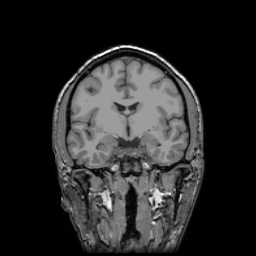
\includegraphics[width=1cm, height=1cm]{data/bert_z_enhanced.png}
            };
            \node[
                anchor=south,
                text=red,
                font=\scriptsize\selectfont\bfseries,
                inner sep=5pt,
                text depth=0
            ] at (-2.5, 0) {
                Too high-dimensional
            };

            \ifnum#1>0
                \draw[] (2.5, 0.075) -- (2.5, -0.075);
                \node[
                    anchor=north,
                    label={[yshift=0.2cm]below:{\scriptsize{$p=1$}}},
                    inner sep=5pt
                ] at (2.5, 0) {
                    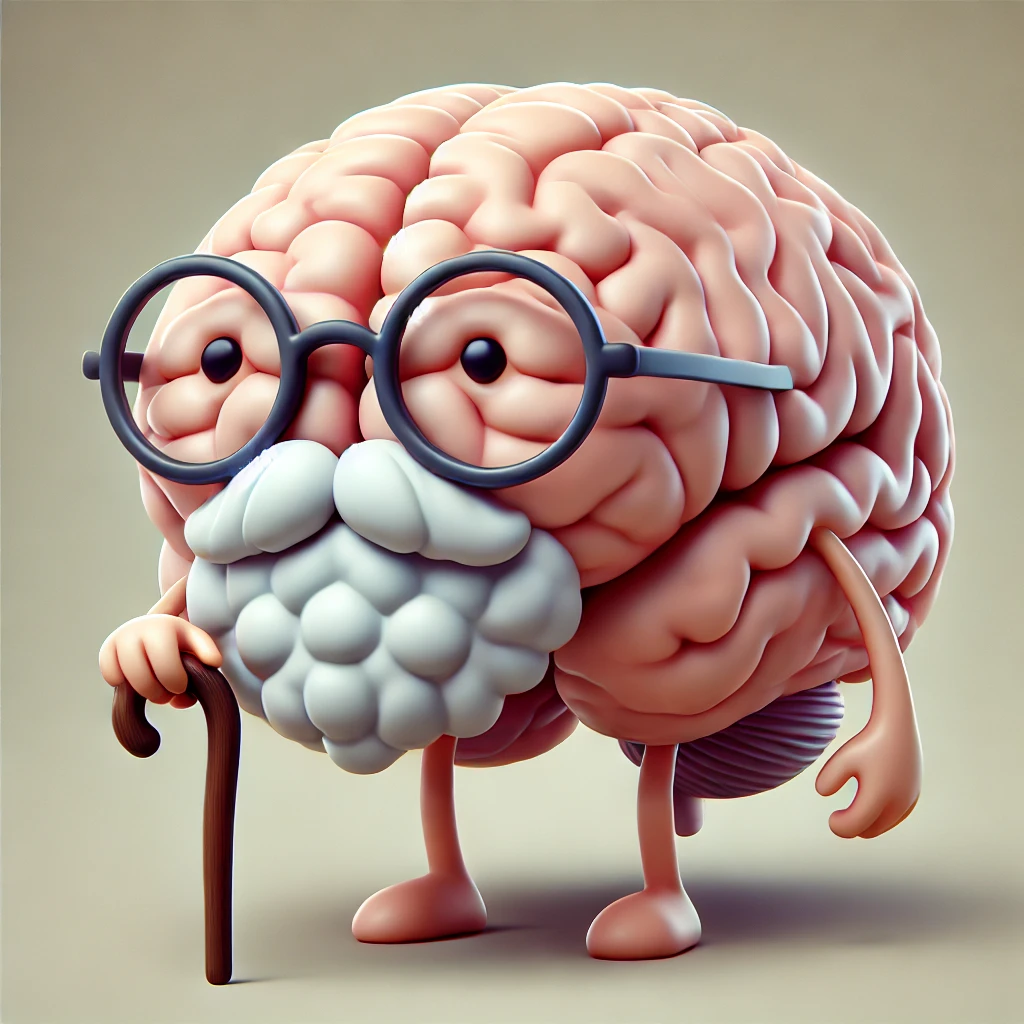
\includegraphics[width=1cm, height=1cm]{data/brainage.png}
                };
                \node[
                    anchor=south,
                    text=red,
                    font=\scriptsize\selectfont\bfseries,
                    inner sep=5pt,
                    text depth=0
                ] at (2.5, 0) {
                    Too abstract
                };
            \fi

            \ifnum#1>1
                \draw[] (1, 0.075) -- (1, -0.075);

                \node[
                    anchor=south,
                    text=cyan,
                    font=\scriptsize\selectfont\bfseries,
                    inner sep=5pt,
                    text depth=0
                ] at (1, 0) {
                    Ideal
                };
            \fi
        \end{tikzpicture}
    }

    \newsavebox{\abstractionmri}
    \sbox{\abstractionmri}{
        \abstractionplot{0}
    }
    \newsavebox{\abstractionbrainage}
    \sbox{\abstractionbrainage}{
        \abstractionplot{1}
    }
    \newsavebox{\abstractionideal}
    \sbox{\abstractionideal}{
        \abstractionplot{2}
    }

    % \begin{frame}{Brain age modelling: Results}
    %     \begin{tikzpicture}
    %         \node[draw=black] at (-5.25, -3.5) {};
    %         \node[draw=black] at (5.25, 3.5) {};

    %         \visible<1>{
    %             \node[] at (0, 0) {
    %                 \usebox{\datasetbox}
    %             };
    %         }

    %         \visible<2>{
    %             \node[] at (0, 0) {
    %                 \usebox{\cnnforward}
    %             };
    %         }

    %         \visible<3>{
    %             \node[] at (0, 0) {
    %                 \usebox{\results}
    %             };
    %         }

    %         \visible<4>{
    %             \node[] at (0, 0) {
    %                 \usebox{\patients}
    %             };
    %         }

    %         \visible<5>{
    %             \node[] at (0, 0) {
    %                 \usebox{\dementiapatients}
    %             };
    %         }

    %         \visible<6>{
    %             \node[] at (0, 0) {
    %                 \usebox{\dementiaclassification}
    %             };
    %         }
    %     \end{tikzpicture}
    % \end{frame}

    % \begin{frame}{Explainable AI: Motivation}
    %     \begin{tikzpicture}
    %         \node[draw=black] at (-5.25, -3.5) {};
    %         \node[draw=black] at (5.25, 3.5) {};
    %         \visible<1>{
    %             \node[] at (0, 0) {
    %                 \usebox{\abstractionmri}
    %             };
    %         }
    %         \visible<2>{
    %             \node[] at (0, 0) {
    %                 \usebox{\abstractionbrainage}
    %             };
    %         }
    %         \visible<3>{
    %             \node[] at (0, 0) {
    %                 \usebox{\abstractionideal}
    %             };
    %         }
    %         \visible<4>{
    %             \node[] at (0, 0) {
    %                 \usebox{\cnntwod}
    %             };
    %         }
    %         \visible<5>{
    %             \node[] at (0, 0) {
    %                 \usebox{\cnnregions}
    %             };
    %         }
    %     \end{tikzpicture}
    % \end{frame}

    \newcommand{\artificialneuron}[5]{
        \node[
            circle,
            fill=#5,
            draw=none,
            minimum size=13pt,
            font=\tiny\selectfont,
            text depth=0,
            inner sep=0pt,
            text=white!90
        ] (#4) at (#1, #2) {#3};
    }
    \newcommand{\connection}[4]{
        \draw[-stealth, line width=1pt,#3] #1 -- #2 #4;
    }

    \newcommand{\mathplot}[1]{
        \begin{tikzpicture}
            \node[draw=black] at (-4, -1.5) {};
            \node[draw=black] at (4, 1.5) {};

            \ifnum#1=0
                \artificialneuron{-0.5}{1}{$n_{00}$}{n00}{black!65}
                \artificialneuron{-0.5}{0.5}{$n_{01}$}{n01}{black!55}
                \artificialneuron{-0.5}{0}{$n_{02}$}{n02}{black!98}

                \artificialneuron{0.5}{0.5}{$n_{10}$}{n10}{black!82}

                \connection{(n00)}{(n10)}{black!45}{node [midway, above, font=\tiny\selectfont, text=black, yshift=-0.05cm] {$w_0$}}
                \connection{(n01)}{(n10)}{black!92}{node [above, font=\tiny\selectfont, text=black, pos=0.35, yshift=-0.11cm] {$w_1$}}
                \connection{(n02)}{(n10)}{black!78}{node [midway, below, font=\tiny\selectfont, text=black, yshift=0.03cm] {$w_2$}}

                \connection{($ (n00.west) - (0.5, 0) $)}{(n00)}{black!65}{}
                \connection{($ (n01.west) - (0.5, 0) $)}{(n01)}{black!55}{}
                \connection{($ (n02.west) - (0.5, 0) $)}{(n02)}{black!98}{}

                \connection{(n10)}{($ (n10.east) + (0.5, 0) $)}{black!82}{}

                \node[anchor=west, font=\tiny\selectfont] at ($ (n10.east) + (0.5, 0) $) {$\hat{y}$};

                \node[anchor=east, font=\tiny\selectfont] at ($ (n00.west) - (0.5, 0) $) {$x_0$};
                \node[anchor=east, font=\tiny\selectfont] at ($ (n01.west) - (0.5, 0) $) {$x_1$};
                \node[anchor=east, font=\tiny\selectfont] at ($ (n02.west) - (0.5, 0) $) {$x_2$};

                \node[font=\footnotesize\selectfont, anchor=north] at (0, -0.25) {
                    $\hat{y}=f\left({\color{red}\sum\limits_i^N w_i \cdot n_{0i}}\right)$
                };
            \fi

            \ifnum#1=1
                \artificialneuron{-0.5}{1}{$n_{00}$}{n00}{red!60!yellow}
                \artificialneuron{-0.5}{0.5}{$n_{01}$}{n01}{red!80!black}
                \artificialneuron{-0.5}{0}{$n_{02}$}{n02}{blue!50!black}

                \artificialneuron{0.5}{0.5}{$n_{10}$}{n10}{red}

                \connection{(n10)}{(n00)}{red!60!yellow}{}
                \connection{(n10)}{(n01)}{red!80!black}{}
                \connection{(n10)}{(n02)}{blue!50!black}{}

                \connection{(n00)}{($ (n00.west) - (0.5, 0) $)}{red!60!yellow}{}
                \connection{(n01)}{($ (n01.west) - (0.5, 0) $)}{red!80!black}{}
                \connection{(n02)}{($ (n02.west) - (0.5, 0) $)}{blue!50!black}{}

                \connection{($ (n10.east) + (0.5, 0) $)}{(n10)}{red}{}

                \node[anchor=west, font=\tiny\selectfont] at ($ (n10.east) + (0.5, 0) $) {$R_{10}$};

                \node[anchor=east, font=\tiny\selectfont] at ($ (n00.west) - (0.5, 0) $) {$R_{00}$};
                \node[anchor=east, font=\tiny\selectfont] at ($ (n01.west) - (0.5, 0) $) {$R_{01}$};
                \node[anchor=east, font=\tiny\selectfont] at ($ (n02.west) - (0.5, 0) $) {$R_{02}$};

                \node[font=\footnotesize\selectfont, anchor=north] at (0, -0.25) {
                    $R_{0i} = \sum\limits_j \dfrac{n_{0i}w_i}{\sum\limits_k n_{0k}w_k}R_{1j}$
                };
            \fi

        \end{tikzpicture}
    }

    \newsavebox{\mathforward}
    \sbox{\mathforward}{
        \mathplot{0}
    }

    \newsavebox{\mathbackward}
    \sbox{\mathbackward}{
        \mathplot{1}
    }

    \begin{frame}{Explainable AI: Methods}
        \begin{tikzpicture}
            \node[] at (-5.25, -3.5) {};
            \node[] at (5.25, 3.5) {};

            \visible<1-3>{
                \node[] at (0, 1.5) {
                    \usebox{\cnnforward}
                };
            }
            \visible<2>{
                \node[anchor=north] at (0, -0.5) {
                    \usebox{\mathforward}
                };
            }
            \visible<3>{
                \node[anchor=north] at (0, -0.5) {
                    \usebox{\mathbackward}
                };
            }
            \visible<4>{
                \node[] at (0, 1.5) {
                    \usebox{\cnnlrp}
                };
            }
        \end{tikzpicture}
    \end{frame}

\end{document}
